%% Revised manuscript (October 2026) for Natural Language Processing Journal, NLP-D-26-00114.
%% Compile with LuaLaTeX (fontspec + Amiri for the Arabic examples). Result tables are generated from the
%% experiment outputs by revision/make_tables.py and included from tables/; figures from revision/make_figures.py.

\documentclass[preprint,12pt,authoryear]{elsarticle}

\usepackage{amssymb}
\usepackage{amsmath}
\usepackage{soul}
\usepackage{xcolor}
\usepackage{cancel}
\usepackage{enumitem}
\usepackage{tcolorbox}
\usepackage{afterpage}
\usepackage{float}
\usepackage{array}
\usepackage{multirow}
\usepackage{ragged2e}
\usepackage{booktabs}
\usepackage{tabularx}
\usepackage{longtable}
\usepackage{rotating}
\usepackage{graphicx}
\usepackage{subcaption}
\usepackage{url}
\graphicspath{{./}{../}{../Figures/}{../Figures_revised/}{Figures/}{Figures_revised/}}

\usepackage{fontspec}
% Arabic excerpts: babel's Unicode bidi algorithm (LuaTeX) so that digits and
% Latin tokens inside right-to-left text keep their own direction.
\usepackage[english,bidi=basic]{babel}
\babelprovide[import]{arabic}
\babelfont[arabic]{rm}[Script=Arabic]{Amiri}
\newcommand{\RTL}[1]{\foreignlanguage{arabic}{#1}}

\usepackage{lineno}
\linenumbers

\begin{document}
\begin{frontmatter}

\begin{titlepage}
\begin{center}
\vspace*{1cm}

\textbf{ \large Arabic News Classification: Lightweight Supervised Models vs. Zero-Shot Large Language Models}

\vspace{1.5cm}

Omar Elgendy$^{a}$ (U20106090@sharjah.ac.ae), Ali Bou Nassif$^a$ (anassif@sharjah.ac.ae), Ashraf Elnagar$^a$ (ashraf@sharjah.ac.ae) \\

\hspace{10pt}

\begin{flushleft}
\small
$^a$ College of Computing and Informatics, University of Sharjah, Sharjah, UAE \\

\vspace{1cm}
\textbf{Corresponding Author:} \\
Ashraf Elnagar \\
Dept of CS, University of Sharjah, Sharjah, UAE \\
Email: ashraf@sharjah.ac.ae

\end{flushleft}
\end{center}
\end{titlepage}

\title{Arabic News Classification: Lightweight Supervised Models vs. Zero-Shot Large Language Models}

\begin{abstract}
This paper compares lightweight supervised classifiers with large language models (LLMs) on seven-way, single-label Arabic news classification using the balanced AlKhaleej subset of the SANAD corpus. The supervised systems use a frozen CAMeLBERT encoder with either a dense classification head or an RBF-kernel SVM; we additionally report full fine-tuning of the encoder and a QLoRA-adapted open-weight LLM (Qwen2.5-7B-Instruct) trained on the same labelled data. The LLMs (GPT-4.1, Claude Haiku 4.5, Gemini 3.8 Flash, DeepSeek V4 Flash and Qwen2.5-7B-Instruct) are evaluated zero-shot and few-shot with deterministic decoding, five semantically equivalent prompts in English and Arabic, and a deterministic, audited label-mapping procedure. All systems are scored on the same deduplicated test split of 6,822 articles, so that comparisons are paired, and every number carries a bootstrap confidence interval. With the full training split, the frozen-encoder heads reach 96.4\% (dense) and 97.1\% (SVM) accuracy at 150 input tokens and 97.5\% and 98.1\% at 512 tokens; full fine-tuning reaches 98.9\% and the QLoRA-adapted LLM 98.5\%. Zero-shot LLMs reach 91.5--92.8\% with a shared weakness on the Religion class (recall 0.71--0.76 against 0.95--0.99 for the supervised systems); prompt wording moves them by 0.3--1.5 points, and few-shot examples help only the weaker models. A learning curve shows that about 100 labelled articles per class are enough for the 0.3\,M-parameter head on a frozen encoder to match the best zero-shot LLM; with 500 per class the head reading 512 wordpieces also exceeds the best few-shot condition on the same articles, while the 150-wordpiece head needs the full training split to do so. Two controlled interventions show that neither family relies on the newspaper dateline or on the opening words of an article. The results characterise when in-domain supervision, even in small amounts, is preferable to zero-shot inference for Arabic text classification, and quantify the cost of each option.
\end{abstract}

\begin{keyword}
   Arabic NLP\sep multi-class text classification\sep lightweight models\sep large language models\sep zero-shot and few-shot evaluation\sep parameter-efficient fine-tuning
\end{keyword}

\end{frontmatter}

\section{Introduction}
\label{intro}

Text classification constitutes a fundamental task within natural language processing, underpinning diverse applications ranging from sentiment analysis \cite{elnagar2021sentiment,bensoltane2022towards,bentrcia2025hybrid} to fake news detection \cite{nassif2022arabic} and hate speech filtering \cite{elgendy2024toxicity, torfa2025enhancing}. Despite substantial progress driven by deep learning methods---most notably transformer-based architectures---significant obstacles persist when dealing with morphologically complex and low-resource languages, Arabic being a prominent example. The language presents particular challenges stemming from its intricate script system, considerable orthographic variability, and elaborate morphological structure, all of which are further complicated by the coexistence of more than twenty regional dialects \cite{helwe2020semi, talafha2020multi}. Although transformer models have advanced the state of Arabic NLP, progress in this domain continues to follow that observed for English and other well-resourced languages despite strong performance reported by supervised Arabic news classification systems \cite{al2019arabic,elnagar2020arabic}. This gap is primarily attributable to the scarcity of annotated data, pronounced domain-specific variation, and class imbalance within available datasets \cite{alhawarat2020superior, almuzaini2020impact}. Such constraints prove particularly acute in scenarios where computational resources are limited or rapid deployment is required, rendering large-scale models impractical.

The Transformer architecture \cite{vaswani2017attention} has given rise to a succession of influential models, including BERT \cite{devlin2018bert}, T5 \cite{roberts2019exploring}, GPT \cite{DBLP:journals/corr/abs-2005-14165}, LLaMA \cite{touvron2023llama}, and Falcon \cite{almazrouei2023falcon}. These systems exhibit robust generalization abilities, performing well even under zero-shot conditions as shown in \cite{DBLP:journals/corr/abs-1909-00161} and \cite{gera2022zero}, and have demonstrated considerable language understanding across varied tasks. Nonetheless, their performance on specific Arabic NLP problems---multi-class news classification among them---has received comparatively little attention \cite{wahdan2024systematic}. Evidence from existing research suggests that models trained for particular tasks frequently surpass general-purpose large language models in terms of both classification accuracy and computational efficiency when processing Arabic text \cite{alruily2023automated, nassif2022arabic}. Yet systematic, paired comparisons between the two paradigms within the Arabic domain remain scarce, and the comparisons that exist rarely control for the amount of supervision each side receives.

This study addresses that gap with a controlled comparison on the balanced AlKhaleej subset of the SANAD dataset, which comprises seven news categories: \textit{Culture}, \textit{Finance}, \textit{Medical}, \textit{Politics}, \textit{Religion}, \textit{Sports}, and \textit{Tech}. On the supervised side we evaluate two lightweight systems built on a frozen CAMeLBERT encoder---a dense classification head and an RBF-kernel support vector machine---together with full fine-tuning of the encoder. On the LLM side we evaluate GPT-4.1, Claude Haiku 4.5, Gemini 3.8 Flash, DeepSeek V4 Flash and the open-weight Qwen2.5-7B-Instruct zero-shot and few-shot, and we adapt Qwen2.5-7B-Instruct to the task with QLoRA on the same labelled data so that the two paradigms can also be compared at equal supervision. All systems are scored on one deduplicated test split, with deterministic decoding, several prompt formulations, an audited output-mapping procedure, confidence intervals and paired significance tests.

This work offers four principal contributions:
\begin{itemize}
    \item A paired benchmark of lightweight supervised classifiers (frozen CAMeLBERT with a dense head or an RBF-SVM, and fully fine-tuned CAMeLBERT) against five contemporary LLMs in zero-shot, few-shot and parameter-efficiently adapted conditions, on a single near-duplicate-aware split of SANAD-AlKhaleej.
    \item A supervised learning curve from 10 to about 4,500 labelled articles per class, which locates the amount of in-domain supervision at which the lightweight systems overtake zero-shot and few-shot LLM inference.
    \item A reproducible LLM evaluation protocol for Arabic classification: pinned model snapshots, deterministic decoding, five semantically equivalent English and Arabic prompts with reported variability, replicate runs, and a deterministic label-mapping procedure whose non-compliance rates are measured and reported.
    \item Two controlled interventions (input length and removal of the newspaper dateline) and a class-level analysis that replace speculative explanations of LLM errors with measured effects, together with a cost analysis of each option.
\end{itemize}

The remainder of this paper proceeds as follows. Section~\ref{rel-works} surveys prior work on Arabic text classification and on the use of large language models under zero-shot, few-shot and parameter-efficient adaptation. Section~\ref{methodology} details the dataset and split, the systems, the LLM evaluation protocol, training configurations, statistical analysis and infrastructure, and documents corrections to the experiments of an earlier version of this work. Section~\ref{results} reports the results. Section~\ref{discussion} interprets them and states the limitations of the study. Section~\ref{conclusion} concludes.

\section{Related Work}
\label{rel-works}

\subsection{Arabic Text Classification}
Arabic text classification has received growing attention due to the Arabic language morphological richness and dialectal diversity. Early efforts relied on traditional machine learning with TF-IDF and n-grams \cite{omar2021multi}. More recent work applied deep neural architectures such as CNNs and RNNs, achieving strong results on news and social media datasets \cite{muaad2022effective,almuzaini2020impact}. For example, SATCDM, a multi-kernel CNN, reached accuracies above 97\% on several benchmarks \cite{alhawarat2020superior}. Despite these gains, traditional neural models remain limited by their dependence on handcrafted features, long training times, and poor cross-dialect generalization.

The release of large Arabic corpora such as SANAD \cite{elnagar2020arabic} enabled systematic evaluation across multiple categories. Models trained on this dataset, including BiGRU and CLSTM, exceeded 96\% accuracy. However, most studies evaluated only deep supervised setups, often under single-label assumptions, without testing emerging large language models \cite{rifai2021arabic,el2022arabic}. News corpora of this kind also contain repeated and near-duplicate stories, which inflate supervised accuracy when a random split places near-identical articles on both sides of the train/test boundary; near-duplicate detection by shingling and similarity thresholds \cite{broder1997resemblance} is the standard remedy and is applied in this work.

\subsection{Arabic Transformer Models}
The introduction of Arabic-specific transformer models marked a turning point in Arabic NLP. AraBERT \cite{helwe2020semi} demonstrated that domain-adapted pretraining on Arabic corpora outperformed multilingual BERT across sentiment, NER, and dialect identification tasks. Successive models such as MARBERT, ARBERT, and QARiB extended coverage to dialectal Arabic. CAMeLBERT, trained on a large clean corpus, showed strong performance on classification and morphological tasks and became a reliable baseline for downstream Arabic applications \cite{yagi2021evaluation,elnagar2023benchmark,nassif2022arabic}.

Benchmarks confirm the importance of Arabic-specific transformers. Nassif et al. \cite{nassif2022arabic} evaluated multiple Arabic and multilingual models on fake news detection. Results showed ARBERT and QARiB outperforming translated datasets and multilingual baselines, reaching up to 98.8\% accuracy. Elgendy et al. \cite{elgendy2024toxicity} extended this line by analyzing bias detection in Arabic texts, highlighting the importance of domain-specific evaluation. These studies emphasize that high-quality pretraining and native datasets remain essential for robust Arabic classification.

\subsection{Zero-Shot, Few-Shot and Parameter-Efficient Use of LLMs}
The rise of large language models (LLMs) such as GPT-3, GPT-4, Claude, Gemini, and DeepSeek introduced the possibility of zero-shot and few-shot learning for Arabic tasks. While multilingual LLMs exhibit strong performance in high-resource languages, their results in Arabic are inconsistent. For example, Zhang and Abdul-Mageed \cite{zhang2019bert} showed that multilingual BERT improves author attribute prediction on Arabic tweets, but dialect classification accuracy remained modest. More broadly, recent evaluations of LLMs on Arabic benchmarks confirm that while they provide competitive results without task-specific training, they still underperform fine-tuned Arabic models in domain-sensitive settings \cite{baniata2023transformer,hossain2024transnet}.

Studies outside Arabic also confirm this trend. Bao et al. \cite{bao2019few} showed that few-shot methods improve classification under limited supervision, but require high-quality prompts and unlabeled data. Comparative works in other low-resource languages reveal that fine-tuned lightweight transformers remain superior to zero-shot LLMs in accuracy and efficiency \cite{ali2022deep}. Recent work cautions that zero-shot evaluation of LLMs on Arabic is highly sensitive to benchmark design, cultural coverage, and category definitions, often leading to misleading conclusions if not carefully controlled \cite{mansour2023sarcasm,al2025need}, and that LLM accuracy can change by several points with semantically irrelevant changes of prompt formatting \cite{sclar2024quantifying}. Two consequences follow for benchmark design: zero-shot results should be reported over several prompt formulations with their variability, and the rules that turn free-form generations into labels are part of the classifier and must be evaluated.

Between zero-shot inference and full fine-tuning lies parameter-efficient adaptation. Low-rank adaptation (LoRA) \cite{hu2022lora} trains small rank-decomposition matrices inside a frozen pretrained model, and QLoRA \cite{dettmers2023qlora} combines it with 4-bit quantization of the base weights so that models of 7B parameters and more can be adapted on a single GPU. Because the adapted model receives exactly the labelled data a supervised classifier receives, such baselines make it possible to separate the effect of model architecture from the effect of the supervision regime; they are included here for that reason.

\sloppy
\subsection{Evaluation and Research Gap}
Existing Arabic benchmarks highlight the performance of supervised models \cite{nassif2022arabic, elgendy2024toxicity}, while recent work has tested LLMs in limited zero-shot contexts. To our knowledge no prior study compares lightweight Arabic transformer classifiers with modern LLMs on the same multi-class news dataset while holding the test set fixed, varying the amount of supervision on both sides (learning curve, few-shot and parameter-efficient adaptation), and reporting the prompt sensitivity and the output-parsing behaviour of the LLMs. Our work addresses this gap on the SANAD-AlKhaleej corpus.

\section{Methodology}
\label{methodology}

\subsection{Dataset and Split}
\label{dataset}

This work utilizes the \textbf{SANAD (Single-Label Arabic News Articles Dataset)} introduced by Einea et al.~\cite{elnagar2020arabic}, a large-scale labeled corpus designed to support Arabic natural language processing tasks such as text classification, document clustering, and word embedding learning. The dataset was compiled using automated scripts that collected articles from three major Arabic news outlets: \textit{AlKhaleej}, \textit{AlArabiya}, and \textit{Akhbarona}. SANAD contains more than 190,000 articles categorized into seven distinct topics: \textit{Culture}, \textit{Finance}, \textit{Medical}, \textit{Politics}, \textit{Religion}, \textit{Sports}, and \textit{Tech}. The only exception is the \textit{AlArabiya} subset, which excludes the \textit{Religion} category due to source limitations. The text is written in Modern Standard Arabic and follows the formal style of journalistic reporting. This work focuses on the AlKhaleej subset, which includes 45,500 articles, equally distributed among the seven categories (Figure~\ref{fig:category_percent}). Each article carries exactly one label, so the task is multi-class, single-label classification. Articles average 369 words (median 258; 90th percentile 779).

\begin{figure}[!ht]
    \centering
    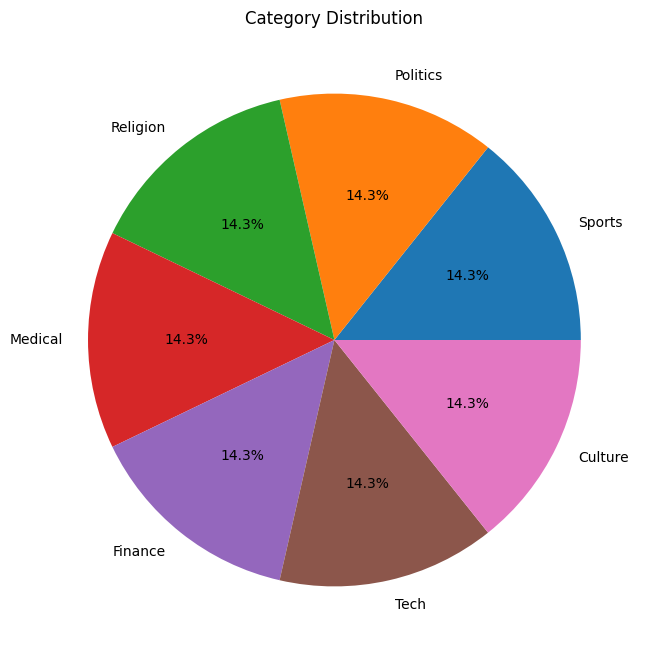
\includegraphics[width=0.6\textwidth]{data categories dist perc.png}
    \caption{Percentage distribution of articles per category in the AlKhaleej subset of SANAD (6,500 articles per class).}
    \label{fig:category_percent}
\end{figure}

\paragraph{Deduplication and near-duplicate-aware split.}
News corpora contain repeated and closely related stories, and a random split can place near-identical articles in training and test, which inflates the accuracy of any system trained on the corpus. We therefore measured and removed this effect. Exact duplicates (identical after removing everything but Arabic letters) number 23 and were dropped. Near-duplicates were identified by TF--IDF cosine similarity over word unigrams and bigrams, with pairs at cosine $\geq 0.8$ joined into clusters by union--find; 183 clusters covering 1,403 articles result, the largest being templated daily stock-market reports in \textit{Finance} (376, 259 and 188 near-identical articles). The corpus was then split 70/15/15 per class with every cluster assigned to a single partition (largest clusters first, each to the partition most below its target size), so that no near-duplicate pair straddles training, validation and test. Table~\ref{tab:split} gives the resulting sizes; no test article has a neighbour at cosine $\geq 0.8$ outside the test set (212 did under a plain random split). Below that threshold some lexical overlap remains by design: 517 test articles (7.6\%) have a neighbour at cosine $\geq 0.5$ in training or validation (307 at $\geq 0.6$, 163 at $\geq 0.7$). These are easy articles for every system, not only for the trained ones: on them the frozen dense head (seed 0) scores 99.8\%, the SVM 99.4\%, full fine-tuning and QLoRA 100\%, and zero-shot GPT-4.1, which has seen no training article, 99.6\%; on the remaining 6,305 articles the same systems score 96.0, 96.9, 98.8, 98.4 and 92.3\%. Excluding them therefore moves every accuracy by 0.1--0.5 points and widens rather than narrows the gap between the dense head and GPT-4.1 (3.8 against 3.5 points); the per-article maximum similarities are released with the split. To quantify what the original random split had been worth, we also trained the frozen-encoder systems on a paper-style random stratified split of the same data: on that split, 10.6\% of test articles have a neighbour at cosine $\geq 0.5$ in the rest of the corpus and the supervised systems are essentially perfect on them, and removing those articles lowers accuracy by 0.3 points. All numbers in this paper use the deduplicated split unless stated otherwise; the split file with per-article checksums is released.

\begin{table}[!ht]
\centering
\caption{The canonical split used by every system: 45{,}477 articles after removing 23 exact duplicates, partitioned 70/15/15 per class so that no near-duplicate cluster (TF--IDF cosine $\geq 0.8$) is divided between partitions.}
\label{tab:split}
\small
\resizebox{\ifdim\width>\textwidth\textwidth\else\width\fi}{!}{%
\begin{tabular}{@{}l r r r@{}}
\toprule
\textbf{Class} & \textbf{Train} & \textbf{Validation} & \textbf{Test} \\
\midrule
Culture & 4,547 & 974 & 974 \\
Finance & 4,548 & 975 & 975 \\
Medical & 4,550 & 975 & 975 \\
Politics & 4,549 & 975 & 975 \\
Religion & 4,541 & 973 & 973 \\
Sports & 4,549 & 975 & 975 \\
Tech & 4,549 & 975 & 975 \\
\midrule
Total & 31,833 & 6,822 & 6,822 \\
\bottomrule
\end{tabular}}
\end{table}


\subsection{Systems}
\label{models}

We evaluate five families of systems. Table~\ref{tab:models_summary} states, for each, exactly which parameters are trained on the SANAD training split; this matters because the lightweight systems keep the encoder frozen.

\begin{table}[!ht]
\centering
\caption{Systems compared in this study and what is trained on the SANAD training split.}
\label{tab:models_summary}
\small
\begin{tabularx}{\textwidth}{@{}>{\raggedright\arraybackslash}p{3.0cm} >{\raggedright\arraybackslash}X >{\raggedleft\arraybackslash}p{1.7cm}@{}}
\toprule
\textbf{System} & \textbf{Description} & \textbf{Trainable params} \\
\midrule
Frozen CAMeLBERT + dense head & CAMeLBERT-MSA (\texttt{bert-base-arabic-\allowbreak camelbert-msa}) \cite{DBLP:journals/corr/abs-2103-06678} as a frozen feature extractor; the 768-dimensional [CLS] vector of the last layer feeds Linear(768$\to$384)--\allowbreak ReLU--\allowbreak Dropout(0.25)--\allowbreak Linear(384$\to$7). Only the head is trained. & 297,991 \\
Frozen CAMeLBERT + RBF-SVM & The same frozen [CLS] embeddings, pre-computed in batches of 32, classified by a support vector machine with RBF kernel ($C=9$, $\gamma=$\,\texttt{scale}; GPU implementation, RAPIDS cuML). No gradient-based training; the encoder is never updated. & -- \\
Fully fine-tuned CAMeLBERT & CAMeLBERT-MSA with a linear classification layer, all layers updated end-to-end. & 109.1\,M \\
Qwen2.5-7B-Instruct + QLoRA & Open-weight LLM \cite{qwen2025qwen25} adapted with QLoRA \cite{dettmers2023qlora,hu2022lora}: 4-bit NF4 base, LoRA rank 16 on all linear projections, trained to emit the category name given the same prompt used for zero-shot evaluation. & 40.4\,M (0.82\%) \\
Zero-/few-shot LLMs & GPT-4.1, Claude Haiku 4.5, Gemini 3.8 Flash, DeepSeek V4 Flash (API) and Qwen2.5-7B-Instruct (local, vLLM \cite{kwon2023vllm}); no parameters are updated; the label is read from the generated text. & 0 \\
\bottomrule
\end{tabularx}
\end{table}

The two frozen-encoder systems are the lightweight classifiers of interest: the encoder is used as a fixed representation and only a small decision function is learned, which keeps training to seconds once the embeddings are computed and makes the systems trivially portable. Keeping the encoder frozen was a deliberate design choice (stability under limited supervision and low cost \cite{AlAyyoub2017, antoun2020, elnagar2023benchmark}), but it also means that any gain these systems show over LLMs must be attributed to a frozen pretrained representation combined with supervised decision-boundary learning, not to task-specific adaptation of the encoder. To make the effect of adapting the encoder measurable, we add full fine-tuning of CAMeLBERT; to make the effect of supervision measurable on the LLM side, we add the QLoRA-adapted Qwen2.5-7B-Instruct and few-shot conditions. Unless stated otherwise the frozen-encoder systems read the first 150 wordpieces of an article, the setting of the original experiments; we also report 512 wordpieces, and the LLMs always receive the full article.

\subsection{LLM Evaluation Protocol}
\label{prompting}

\paragraph{Models and snapshots.} Table~\ref{tab:llm_snapshots} lists the exact model identifiers, routes and evaluation dates. Three of the four API models of an earlier version of this study (Claude 3.5 Haiku, Gemini 2.0 Flash and DeepSeek V3) have since been retired by their providers; the revision uses the closest same-tier successors and reports them under their own names. The identifier returned by the API, the raw output, the finish reason, token counts and latency are stored for every request.

\begin{table}[!ht]
\centering
\caption{LLM snapshots, routes and decoding settings. All runs on 16 October 2026. Temperature 0, top-p 1, seed 42 where accepted, 60-second timeout; retries (at most six, exponential back-off) only on rate-limit and server errors, all other failures recorded as errors. Prompt caching was enabled where offered; it affects cost, not outputs.}
\label{tab:llm_snapshots}
\small
\begin{tabularx}{\textwidth}{@{}>{\raggedright\arraybackslash}p{2.0cm} >{\raggedright\arraybackslash}p{4.1cm} >{\raggedright\arraybackslash}p{2.6cm} >{\raggedright\arraybackslash}X@{}}
\toprule
\textbf{Model} & \textbf{Identifier (served model)} & \textbf{Route} & \textbf{Output budget / notes} \\
\midrule
GPT-4.1 & \texttt{openai/gpt-4.1} (gpt-4.1) & OpenRouter, pinned to OpenAI, fallbacks disabled & 16 tokens \\
Claude Haiku 4.5 & \texttt{anthropic/\allowbreak claude-haiku-4.5} (claude-haiku-4-5-\allowbreak 20251001) & OpenRouter, pinned to Anthropic & 16 tokens \\
Gemini 3.8 Flash & \texttt{google/\allowbreak gemini-3.8-flash} & OpenRouter, pinned to Google AI Studio & 256 tokens; reasoning cannot be disabled on this endpoint and runs at minimal effort (0--60 reasoning tokens per request, logged) \\
DeepSeek V4 Flash & \texttt{deepseek-ai/\allowbreak DeepSeek-V4-\allowbreak Flash-0731} & Together AI (serverless) & 16 tokens; reasoning disabled \\
Qwen2.5-7B-Instruct & \texttt{Qwen/\allowbreak Qwen2.5-7B-Instruct}, bf16 & local, vLLM 16k context & 16 tokens; also the QLoRA base \\
\bottomrule
\end{tabularx}
\end{table}

\paragraph{Prompts.} Each model is evaluated with five semantically equivalent prompts: three in English (\texttt{en\_v1}, the wording used by the code of the original experiments, which the submitted manuscript had paraphrased; \texttt{en\_v2}, the primary prompt; \texttt{en\_v3}) and two in Arabic (\texttt{ar\_v1}, \texttt{ar\_v2}). All present the seven category names and ask for exactly one of them; the full texts are given in \ref{app:prompts}. The primary prompt is
\begin{quote}\small
\textit{System: You are a precise news-topic classifier for Modern Standard Arabic.}\\
\textit{User: Classify the Arabic news article below into exactly one of these categories: ['Culture', 'Finance', 'Medical', 'Politics', 'Religion', 'Sports', 'Tech']. Respond with the category name only, copied exactly from the list, with no explanation.} [examples] \textit{Article:} [text] \textit{Category:}
\end{quote}
In the few-shot conditions, $k\in\{1,2\}$ exemplars per class are inserted before the article: the first $k$ articles per class of a fixed random ranking of the training split, truncated to 120 words, in a fixed shuffled order, identical for every model. The examples and the instruction form a prefix shared by all requests of a run, which allows provider-side prompt caching.

\paragraph{Label mapping.} The generated text is mapped to a label by a fixed ordered rule list with no random component: (1) exact match to one of the seven labels; (2) match after removing surrounding punctuation, quotes, brackets and a leading ``Class:''/``Category:'' and ignoring case (\textit{``sports.''} $\to$ Sports); (3) match to a fixed list of Arabic label names (\textit{\RTL{رياضة}} $\to$ Sports); (4) otherwise, if exactly one label (English or Arabic) occurs anywhere in the output, that label (\textit{``The class is Finance''} $\to$ Finance). Outputs that mention two labels are scored as ambiguous and outputs that mention none (including empty outputs and API errors) as unmapped; both count as errors. A lenient variant that also accepts common synonyms (Economy $\to$ Finance, Health $\to$ Medical) is reported as a sensitivity analysis; it changes no accuracy in this paper by more than 0.2 points. The share of outputs resolved by each rule is reported per model in Section~\ref{sec:robustness}.

\paragraph{Evaluation sets.} The primary prompt is run on the full test split of 6,822 articles for every model, and these are the numbers of the main table. The prompt variants, the few-shot conditions, the controls and a replicate run are evaluated on a fixed stratified subset of 700 test articles (100 per class; the list is released) to keep the API cost of the sweeps proportionate; at this size the standard error of an accuracy is about 0.7 points. The subset is easier for the LLMs than the full test set: with the primary prompt every model scores higher on it, by 1.4 (Qwen2.5-7B), 1.8 (Claude Haiku 4.5, DeepSeek V4 Flash), 2.0 (Gemini 3.8 Flash) and 2.6 points (GPT-4.1), whereas the supervised systems score within one point of their full-set accuracy on it, in both directions. Subset numbers are therefore only compared with other subset numbers: prompt-to-prompt, few-shot-to-zero-shot and control differences, and, where a cross-family comparison is made, the supervised systems re-scored on the same 700 articles. The main comparison and the learning curve use the full set.

\subsection{Training Configuration}
\label{training}

Table~\ref{tab:hyperparameters} lists the training configuration of every trained system. The dense head is trained with AdamW (learning rate $10^{-3}$, weight decay 0.01, batch 32, cross-entropy loss) for at most 50 epochs with early stopping on validation loss (patience 5, best checkpoint restored); this recipe was fixed before any test evaluation because the learning curve needs one that works from 70 to 31,833 training articles. The configuration of the original experiments (learning rate $5\times10^{-5}$, 10 epochs, no early stopping, one seed) is reported next to it in Table~\ref{tab:main}: on the same split it reaches 96.8\% (validation accuracy 97.1\% against 96.9\% for the early-stopped recipe), 0.4 points above the headline configuration, so the headline numbers of the dense head are, if anything, conservative. The SVM is fit once on the pre-computed training embeddings. Full fine-tuning uses AdamW with learning rate $2\times10^{-5}$, a linear schedule with 6\% warm-up, batch 32, mixed precision, 512 wordpieces, at most three epochs with early stopping on validation loss. QLoRA uses a 4-bit NF4 base with double quantization, LoRA rank 16, $\alpha=32$, dropout 0, on all attention and MLP projections, learning rate $2\times10^{-4}$ with a cosine schedule, batch 16, sequences up to 1,024 tokens (articles truncated to 350 words for training only), and one epoch on the full training split (two and three epochs at 1,000 and 100 articles per class), implemented with Unsloth \cite{unsloth2024}. Every supervised configuration is trained with three seeds (which also select the nested learning-curve subsets) unless stated otherwise; full fine-tuning on the full split uses one seed.

\begin{table}[!ht]
\centering
\caption{Training configuration of the supervised and adapted systems.}
\label{tab:hyperparameters}
\small
\resizebox{\ifdim\width>\textwidth\textwidth\else\width\fi}{!}{%
\begin{tabular}{@{}l l l l l@{}}
\toprule
\textbf{Setting} & \textbf{Dense head} & \textbf{RBF-SVM} & \textbf{Full fine-tuning} & \textbf{QLoRA (Qwen2.5-7B)} \\
\midrule
Encoder / base & CAMeLBERT-MSA, frozen & CAMeLBERT-MSA, frozen & CAMeLBERT-MSA, all layers & Qwen2.5-7B-Instruct, 4-bit NF4 \\
Input length & 150 or 512 wordpieces & 150 or 512 wordpieces & 512 wordpieces & $\leq$1,024 tokens \\
Trainable parameters & 297,991 & -- & 109.1\,M & 40.4\,M (rank 16, $\alpha$=32) \\
Optimizer / LR & AdamW, $10^{-3}$ (orig.\ $5\times10^{-5}$) & -- & AdamW, $2\times10^{-5}$, linear, 6\% warm-up & AdamW (8-bit), $2\times10^{-4}$, cosine \\
Batch size & 32 & 32 (embedding extraction) & 32 & 16 \\
Epochs / stopping & $\leq$50, early stop (val.\ loss, patience 5) & single fit & $\leq$3, early stop (patience 1) & 1 (all), 2 (1,000/cls), 3 (100/cls) \\
Regularization & dropout 0.25, weight decay 0.01 & $C=9$, $\gamma=$\,scale & weight decay 0.01, grad.\ clip 1.0 & -- \\
Seeds & 3 & 3 & 3 (1 on full split) & 1 \\
\bottomrule
\end{tabular}}
\end{table}

\subsection{Evaluation and Statistical Analysis}
\label{stats}

We report accuracy and macro-averaged precision, recall and F1 on the test split, per-class recall, and confusion matrices. Every accuracy carries a 95\% bootstrap confidence interval over test articles (2,000 resamples); supervised numbers are means over seeds with their standard deviation. Because all systems are scored on the same articles, headline differences are tested with McNemar's exact test on paired predictions \cite{dietterich1998approximate}, and the paired bootstrap of the accuracy difference is reported alongside. Prompt sensitivity is reported as the mean, standard deviation and range over the five prompts; residual nondeterminism is measured by a second identical pass of the primary prompt. The learning curve uses nested training subsets of 10, 50, 100, 500, 1,000 and all articles per class, drawn by a fixed per-seed ranking of the training split so that smaller subsets are contained in larger ones. Two controlled interventions probe lexical shortcuts: (a) input length, by comparing 150 and 512 wordpieces for the frozen encoder and the first 100 words against the full article for the LLMs; and (b) the newspaper dateline (\textit{\RTL{دبي: «الخليج»}}), a city-and-source prefix present in 12\% of articles and strongly class-skewed (40\% of \textit{Medical} and 0.1\% of \textit{Sports} articles), which we remove from the test articles, and additionally from the training articles for the dense head, to measure whether any system uses it as a cue.

\subsection{Infrastructure and Reproducibility}
\label{infrastructure}

Supervised training, full fine-tuning, QLoRA and the open-weight LLM inference ran on one NVIDIA A100-PCIE-40GB (cloud instance) with CUDA 13.2, Python 3.12, PyTorch 2.14, Transformers 5.20, RAPIDS cuML for the GPU SVM, Unsloth, PEFT and TRL for QLoRA, and vLLM for open-weight inference. API models were called through the routes in Table~\ref{tab:llm_snapshots}; all API runs took place on 16 October 2026 and all GPU runs on 16--17 October 2026, and every run is logged publicly on Weights \& Biases. The split file with per-article checksums, the deduplication clusters, the 700-article evaluation subset, all per-article predictions and raw LLM outputs, the QLoRA budgets, and the complete code are released at \url{https://github.com/omaratef3221/Bert-rbf-arabic-text-classification} (folder \texttt{revision/}).

\subsection{Corrections to the Originally Reported Experiments}
\label{corrections}

While re-implementing the evaluation pipeline for this version we found three defects in the experiments reported in an earlier version of this paper; we document them because the affected numbers were replaced. First, the result previously reported for Claude 3.5 Haiku (75\% accuracy, \textit{Religion} recall 0) was a parsing artefact: the run requested a single output token, the model often answered in Arabic, the returned token was a word prefix carrying no label, and the post-processing code had no rule for the \textit{Religion} class and assigned a random other label to unrecognised outputs. With an adequate output budget the same model reaches 92--93\% and \textit{Religion} recall 0.76; the interpretation of that result as a cultural or alignment limitation has been withdrawn. Second, the random split had been drawn without a fixed seed in each evaluation, so the systems had been scored on different test samples; the present version uses one split for all systems. Third, one run reported as GPT-4.1 had been executed with a smaller model, and the API models had been decoded at default (non-zero) temperature; all runs are now on pinned snapshots with deterministic decoding. In addition, the prompt printed in the submitted manuscript was a paraphrase of the one the code used; the exact wording is now given verbatim as \texttt{en\_v1} in \ref{app:prompts}.

\section{Experimental Results}
\label{results}

\subsection{Main Results}
\label{sec:main}

Table~\ref{tab:main} reports all systems on the shared test split. The frozen-encoder systems reach 96.4\% (dense head) and 97.1\% (RBF-SVM) at 150 wordpieces and 97.5\% and 98.1\% at 512, with narrow confidence intervals and near-identical macro precision, recall and F1, as expected on a balanced test set. Adapting the parameters of a large model to the task gives the best results: full fine-tuning of CAMeLBERT reaches 98.9\%, and the QLoRA-adapted Qwen2.5-7B-Instruct 98.5\% with the full training split and 98.4\% with 1,000 articles per class. The zero-shot LLMs lie within 1.3 points of each other, from 92.8\% (GPT-4.1) to 91.5\% (Gemini 3.8 Flash and DeepSeek V4 Flash); the 7B open-weight model is clearly weaker zero-shot (85.2\% with the primary prompt, 89.2\% with the original wording) but closes the gap once adapted.

\begin{table}[!ht]
\centering
\caption{Main results on the shared, deduplicated test split (6{,}822 articles). Accuracy is the mean over training seeds ($\pm$ standard deviation where more than one seed was run) with the 95\,\% bootstrap confidence interval of a single run; precision, recall and F1 are macro-averaged over the seven classes, in percent. ``Trainable'' is the number of parameters updated on the SANAD training split. All LLMs use the primary prompt with deterministic decoding.}
\label{tab:main}
\small
\resizebox{\ifdim\width>\textwidth\textwidth\else\width\fi}{!}{%
\begin{tabular}{@{}l r r l r r r@{}}
\toprule
\textbf{System} & \textbf{Trainable} & \textbf{Accuracy} & \textbf{95\,\% CI} & \textbf{Prec.} & \textbf{Rec.} & \textbf{F1} \\
\midrule
Frozen CAMeLBERT + dense head (150 tok.) & 0.30\,M & 96.4$\pm$0.2 & [95.9, 96.8] & 96.4 & 96.4 & 96.4 \\
Frozen CAMeLBERT + dense head (150 tok., original recipe, 1 seed) & 0.30\,M & 96.8 & [96.4, 97.2] & 96.8 & 96.8 & 96.8 \\
Frozen CAMeLBERT + RBF-SVM (150 tok.) & -- & 97.1$\pm$0.0 & [96.7, 97.5] & 97.1 & 97.1 & 97.1 \\
Frozen CAMeLBERT + dense head (512 tok.) & 0.30\,M & 97.5$\pm$0.1 & [97.1, 97.8] & 97.6 & 97.5 & 97.5 \\
Frozen CAMeLBERT + RBF-SVM (512 tok.) & -- & 98.1$\pm$0.0 & [97.8, 98.4] & 98.1 & 98.1 & 98.1 \\
Fully fine-tuned CAMeLBERT (512 tok.) & 109.1\,M & 98.9 & [98.7, 99.1] & 98.9 & 98.9 & 98.9 \\
\addlinespace
Qwen2.5-7B-Instruct + QLoRA, all training data & 40.4\,M & 98.5 & [98.2, 98.8] & 98.5 & 98.5 & 98.5 \\
Qwen2.5-7B-Instruct + QLoRA, 1{,}000 / class & 40.4\,M & 98.4 & [98.1, 98.7] & 98.4 & 98.4 & 98.4 \\
Qwen2.5-7B-Instruct + QLoRA, 100 / class & 40.4\,M & 95.7 & [95.2, 96.2] & 95.8 & 95.7 & 95.7 \\
\addlinespace
GPT-4.1, zero-shot & 0 & 92.8 & [92.2, 93.4] & 93.2 & 92.8 & 92.7 \\
Claude Haiku 4.5, zero-shot & 0 & 92.0 & [91.4, 92.7] & 92.5 & 92.0 & 91.9 \\
Gemini 3.8 Flash, zero-shot & 0 & 91.5 & [90.8, 92.1] & 92.5 & 91.5 & 91.4 \\
DeepSeek V4 Flash, zero-shot & 0 & 91.5 & [90.9, 92.1] & 92.3 & 91.5 & 91.4 \\
Qwen2.5-7B-Instruct, zero-shot & 0 & 85.2 & [84.3, 86.0] & 87.9 & 85.2 & 84.9 \\
\bottomrule
\end{tabular}}
\end{table}


The headline differences are all significant on paired predictions: the frozen dense head exceeds GPT-4.1 by 3.5 points (95\% CI 2.9--4.2, McNemar $p=9\times10^{-27}$; 376 articles right only for the head, 137 right only for GPT-4.1), the SVM by 4.3 points ($p=2\times10^{-37}$), the QLoRA-adapted model by 5.7 points ($p<10^{-80}$); GPT-4.1 exceeds Claude Haiku 4.5 by 0.8 points ($p=3\times10^{-4}$); full fine-tuning exceeds the frozen dense head by 2.6 points ($p=8\times10^{-34}$) and the QLoRA model by 0.4 points ($p=0.015$); and 512 input tokens improve the dense head over 150 by 1.1 points ($p=3\times10^{-7}$). On the original random split the frozen systems score 96.8\% and 97.2\%, so deduplication cost 0.1--0.4 points, consistent with the leakage measurement in Section~\ref{dataset}.

\subsection{Class-Level Analysis}
\label{sec:classes}

Figure~\ref{fig:confusion} shows the confusion matrices of the frozen dense head and of GPT-4.1, and Table~\ref{tab:perclass} the per-class recall of all systems. The two families err in different places. The supervised head's residual errors are spread thinly, with the two largest cells \textit{Religion}$\to$\textit{Culture} (44 of 973) and \textit{Tech}$\to$\textit{Finance} (28 of 975); full fine-tuning removes most of them (\textit{Religion} recall 0.99). The zero-shot LLMs are at or above the supervised systems on \textit{Culture}, \textit{Finance} and \textit{Sports} but lose 4--13 points on \textit{Medical}, \textit{Politics} and \textit{Tech}, and 20--25 points on \textit{Religion}, where GPT-4.1 routes 172 of 973 articles to \textit{Culture} and smaller numbers to \textit{Medical} and \textit{Politics}. The pattern is the same for all four API models (\textit{Religion} recall 0.71--0.76) and more pronounced for Qwen2.5-7B (0.53), so it is a property of the task framing rather than of one model. The articles involved are typically historical or devotional pieces that the publisher files under \textit{Religion} and that a general-purpose model can defensibly read as cultural; the supervised systems learn this publisher-specific convention from the labels, which the LLMs cannot know.

\begin{figure}[!ht]
\centering
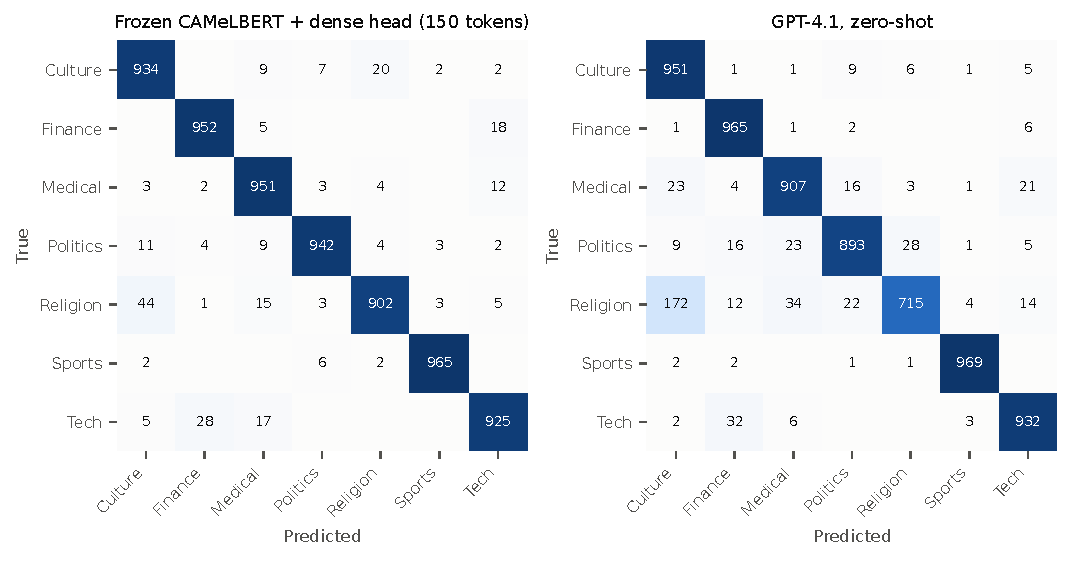
\includegraphics[width=\textwidth]{fig_confusion.pdf}
\caption{Confusion matrices on the shared test split (rows: true class; columns: predicted class; counts). Left: frozen CAMeLBERT with the dense head (150 wordpieces, seed 0). Right: GPT-4.1 zero-shot with the primary prompt.}
\label{fig:confusion}
\end{figure}

\begin{table}[!ht]
\centering
\caption{Per-class recall on the shared test split (975 articles per class, 973--975 after deduplication). Supervised systems: mean over seeds; LLMs: zero-shot, primary prompt. Religion is the weakest class for every zero-shot LLM and the only class where the gap to the supervised systems exceeds 20 points.}
\label{tab:perclass}
\small
\resizebox{\ifdim\width>\textwidth\textwidth\else\width\fi}{!}{%
\begin{tabular}{@{}l rrrr rrrr@{}}
\toprule
 & \multicolumn{4}{c}{\textbf{Supervised / adapted}} & \multicolumn{4}{c}{\textbf{Zero-shot LLMs}} \\
\cmidrule(lr){2-5}\cmidrule(lr){6-9}
\textbf{Class} & Dense 150 & SVM 150 & Fine-tuned & QLoRA all & GPT-4.1 & Claude 4.5 & Gemini 3.8 & DeepSeek V4 \\
\midrule
Culture & 0.939 & 0.945 & 0.994 & 0.968 & 0.976 & 0.977 & 0.990 & 0.975 \\
Finance & 0.977 & 0.974 & 0.977 & 0.990 & 0.990 & 0.992 & 0.998 & 0.993 \\
Medical & 0.972 & 0.972 & 0.982 & 0.989 & 0.930 & 0.896 & 0.920 & 0.875 \\
Politics & 0.970 & 0.985 & 0.993 & 0.993 & 0.916 & 0.939 & 0.949 & 0.974 \\
Religion & 0.955 & 0.965 & 0.986 & 0.980 & 0.735 & 0.741 & 0.716 & 0.705 \\
Sports & 0.992 & 0.992 & 0.998 & 0.998 & 0.994 & 0.991 & 0.992 & 0.984 \\
Tech & 0.944 & 0.964 & 0.994 & 0.977 & 0.956 & 0.906 & 0.838 & 0.899 \\
\midrule
Macro F1 & 0.964 & 0.971 & 0.989 & 0.985 & 0.927 & 0.919 & 0.914 & 0.914 \\
\bottomrule
\end{tabular}}
\end{table}


\subsection{How Much Supervision Does the Lightweight System Need?}
\label{sec:lc}

Figure~\ref{fig:lc} and Table~\ref{tab:lc} report the learning curve. With 10 labelled articles per class the frozen dense head reaches 82.5\% (88.4\% at 512 wordpieces), with 50 per class 90.9\% (94.2\%), and with 100 per class 92.9\% (95.1\%), which already matches or exceeds the best zero-shot LLM (92.8\%). The few-shot conditions were measured on the 700-article subset, so we compare them with the supervised systems scored on the same 700 articles: at 500 per class the 512-wordpiece head reaches 96.7\% there against 95.3\% for the best few-shot condition (Gemini 3.8 Flash, $k=2$), whereas the 150-wordpiece head (94.4\% at 500 and 95.0\% at 1,000 per class) only passes it with the full training split (96.5\%; the RBF-SVM does so from 1,000 per class, 95.7\%). On the full test set the curves continue to rise to 96.4\% / 97.5\% with the full split. The RBF-SVM follows the same curve within one point. Full fine-tuning and QLoRA start higher and saturate earlier: 96.6\% and 95.7\% with 100 per class, 98.4\% for both with 1,000 per class, and 98.9\% and 98.5\% with the full split. In other words, the crossover between zero-shot LLM inference and in-domain supervision on this task lies at roughly 100 labelled articles per class for a 0.3\,M-parameter head, and the ceiling of the task is reached with about 1,000 per class by any adapted model.

\begin{figure}[!ht]
\centering
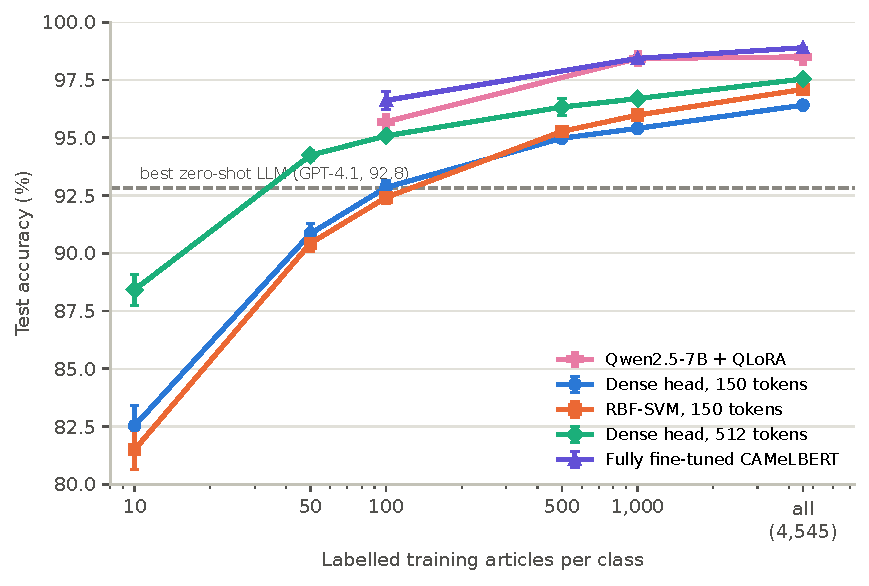
\includegraphics[width=0.9\textwidth]{fig_learning_curve.pdf}
\caption{Learning curve on the shared test split: accuracy as a function of labelled training articles per class (log scale; mean and standard deviation over three seeds; nested subsets). The horizontal line marks the best zero-shot LLM on the full test set; the few-shot conditions were measured on the 700-article subset and are compared with the supervised systems on that subset in the text.}
\label{fig:lc}
\end{figure}

\begin{table}[!ht]
\centering
\caption{Learning curve: test accuracy (\%) as a function of the number of labelled training articles per class (mean $\pm$ standard deviation over three seeds; ``all'' = the full training split, about 4{,}545 per class). Nested subsets drawn with a fixed ranking of the training split. For reference, the best zero-shot LLM reaches 92.8\,\% on the full test set; the best few-shot condition, 95.3\,\% (Table~\ref{tab:prompts}), was measured on the 700-article subset and is compared with the supervised systems on that subset in the text.}
\label{tab:lc}
\small
\resizebox{\ifdim\width>\textwidth\textwidth\else\width\fi}{!}{%
\begin{tabular}{@{}l rrrrrr@{}}
\toprule
\textbf{System} & \textbf{10} & \textbf{50} & \textbf{100} & \textbf{500} & \textbf{1{,}000} & \textbf{all} \\
\midrule
Dense head, 150 tokens & 82.5$\pm$0.9 & 90.9$\pm$0.4 & 92.9$\pm$0.3 & 95.0$\pm$0.1 & 95.4$\pm$0.1 & 96.4$\pm$0.2 \\
RBF-SVM, 150 tokens & 81.5$\pm$0.8 & 90.4$\pm$0.4 & 92.4$\pm$0.3 & 95.3$\pm$0.2 & 96.0$\pm$0.1 & 97.1$\pm$0.0 \\
Dense head, 512 tokens & 88.4$\pm$0.7 & 94.2$\pm$0.2 & 95.1$\pm$0.0 & 96.3$\pm$0.4 & 96.7$\pm$0.1 & 97.5$\pm$0.1 \\
Fully fine-tuned CAMeLBERT & -- & -- & 96.6$\pm$0.4 & -- & 98.4$\pm$0.1 & 98.9 \\
Qwen2.5-7B + QLoRA & -- & -- & 95.7 & -- & 98.4 & 98.5 \\
\bottomrule
\end{tabular}}
\end{table}


\subsection{Prompt Robustness, Few-Shot Conditions and Output Mapping}
\label{sec:robustness}

Table~\ref{tab:prompts} and Figure~\ref{fig:prompts} report the sweeps on the fixed 700-article subset. Across the five prompt formulations the standard deviation of accuracy is 0.5 points for GPT-4.1, 0.7 for Claude Haiku 4.5 and 0.3 for Gemini 3.8 Flash, 1.5 for DeepSeek V4 Flash and 2.5 for Qwen2.5-7B; the Arabic prompts are neither systematically better nor worse than the English ones (for DeepSeek they are the best two, for Claude the lowest two). The ranking of the API models is the same under every prompt. A second identical pass of the primary prompt reproduces every model's accuracy to within 0.1 points, so decoding at temperature 0 is effectively deterministic and the variability that matters is the one across prompt wordings. Few-shot examples help the weaker models and not the stronger ones: with two exemplars per class Gemini gains 1.9 points, DeepSeek 1.1 and Qwen2.5-7B 5.0 (with one exemplar per class), while GPT-4.1 loses 1.0 point and Claude 0.4; on the same 700 articles the best few-shot condition (95.3\%) is below the 512-wordpiece dense head trained on 500 articles per class (96.7\%) and above the 150-wordpiece head at that size (94.4\%; Section~\ref{sec:lc}).

\begin{table}[!ht]
\centering
\caption{LLM robustness and in-context conditions on the fixed 700-article evaluation subset (100 per class; identical articles for every model; accuracy in \%). ``Primary'' is the main prompt; the spread is over five semantically equivalent prompts (three English, two Arabic); $k$ exemplars per class are drawn from the training split; ``Repeat'' is a second identical pass of the primary prompt at temperature 0; ``No dateline'' removes the newspaper dateline from every article; ``100 words'' truncates each article to its first 100 words. Qwen2.5-7B zero-/few-shot runs used the full test set and are reported on the same 700 articles.}
\label{tab:prompts}
\small
\setlength{\tabcolsep}{4pt}
\resizebox{\ifdim\width>\textwidth\textwidth\else\width\fi}{!}{%
\begin{tabular}{@{}l r r r rr r r r@{}}
\toprule
 & & \multicolumn{2}{c}{\textbf{5 prompts}} & \multicolumn{2}{c}{\textbf{Few-shot}} & \multicolumn{3}{c}{\textbf{Controls}} \\
\cmidrule(lr){3-4}\cmidrule(lr){5-6}\cmidrule(lr){7-9}
\textbf{Model} & \textbf{Primary} & \textbf{mean$\pm$std} & \textbf{min--max} & $k=1$ & $k=2$ & \textbf{Repeat} & \textbf{No dateline} & \textbf{100 words} \\
\midrule
GPT-4.1 & 95.4 & 95.2$\pm$0.5 & 94.7--95.9 & 94.4 & 94.4 & 95.4 & 95.4 & 94.4 \\
Claude Haiku 4.5 & 93.9 & 92.9$\pm$0.7 & 92.1--93.9 & 92.9 & 93.4 & 93.9 & 93.7 & 93.3 \\
Gemini 3.8 Flash & 93.4 & 93.1$\pm$0.3 & 92.7--93.4 & 94.9 & 95.3 & 93.4 & 93.6 & 92.4 \\
DeepSeek V4 Flash & 93.3 & 92.2$\pm$1.5 & 89.9--93.7 & 94.3 & 94.4 & 93.4 & 92.9 & 92.6 \\
Qwen2.5-7B-Instruct & 86.6 & 87.4$\pm$2.5 & 84.9--90.3 & 91.6 & 88.9 & -- & -- & -- \\
\bottomrule
\end{tabular}}
\end{table}


\begin{figure}[!ht]
\centering
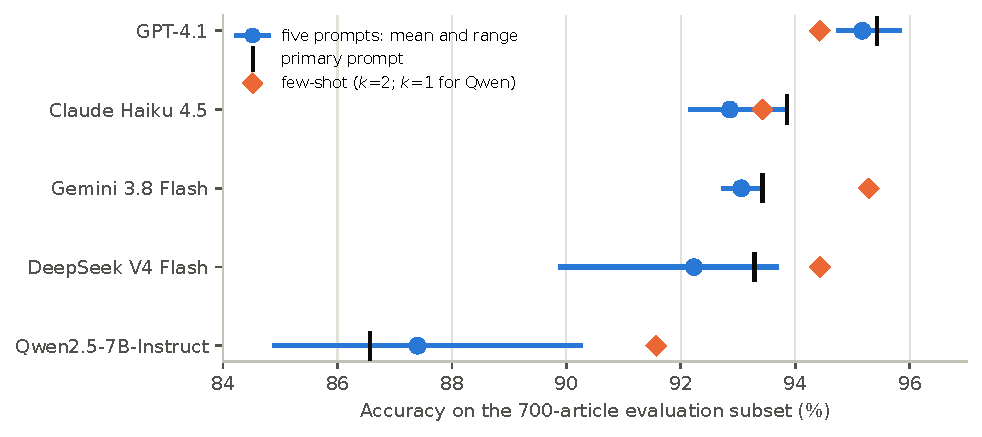
\includegraphics[width=0.85\textwidth]{fig_prompt_robustness.pdf}
\caption{Prompt sensitivity and few-shot effect on the 700-article evaluation subset. For each model: mean and range of zero-shot accuracy over five semantically equivalent prompts, the primary prompt, and the few-shot condition.}
\label{fig:prompts}
\end{figure}

Table~\ref{tab:mapping} audits the label-mapping step over every run of each model. All four API models return a bare label for most requests, and the share of unmapped outputs on the full test set is 0.00\% (GPT-4.1), 0.04\% (Claude), 0.06\% (Gemini) and 0.01\% (DeepSeek), at most four articles. The resolved share shows which models deviate from the requested format and how: under one English prompt Claude Haiku 4.5 wrapped the label in surrounding text in 55\% of answers, under the Arabic prompts GPT-4.1 answered with the Arabic label name in 8--12\% of cases and Gemini added formatting to 97\% of answers; all of these were resolved by the fixed rules, and none of them changed accuracy by more than the unmapped rate. Qwen2.5-7B zero-shot produces 0.3--0.7\% unmapped outputs (a free continuation of the article instead of a label); after QLoRA the model answers with a bare label in every case. The mapping step is therefore not a hidden source of the differences reported above.

\begin{table}[!ht]
\centering
\caption{Audit of the label-mapping step over all runs of each model (zero-shot prompts, few-shot, controls and repeats, plus the three QLoRA evaluations on the full test set; the DeepSeek V4 Flash subset runs cover a 1,400-article superset of the evaluation subset). ``Exact'' outputs are the bare label string; ``resolved'' outputs contained extra formatting, an Arabic label name, or a sentence with exactly one label and were mapped by the fixed rules; unmapped (no label, two labels, or an API error) outputs are scored as errors. All shares are percentages of the outputs of the model; ``worst run'' is the highest share in any single run.}
\label{tab:mapping}
\small
\resizebox{\ifdim\width>\textwidth\textwidth\else\width\fi}{!}{%
\setlength{\tabcolsep}{4pt}%
\begin{tabular}{@{}l r r r r r r r@{}}
\toprule
\textbf{Model} & \textbf{Runs} & \textbf{Outputs} & \textbf{Exact} & \textbf{Resolved} & \textbf{Resolved, worst run} & \textbf{Unmapped} & \textbf{Unmapped, worst run} \\
\midrule
GPT-4.1 & 10 & 13,122 & 92.7 & 7.3 & 100.0 & 0.00 & 0.00 \\
Claude Haiku 4.5 & 10 & 13,122 & 97.0 & 3.0 & 55.4 & 0.02 & 0.04 \\
Gemini 3.8 Flash & 10 & 13,122 & 94.8 & 5.2 & 97.3 & 0.04 & 0.14 \\
DeepSeek V4 Flash & 10 & 24,844 & 99.9 & 0.1 & 0.6 & 0.02 & 0.07 \\
Qwen2.5-7B (zero-/few-shot) & 7 & 47,754 & 96.6 & 3.4 & 9.0 & 0.51 & 1.00 \\
Qwen2.5-7B + QLoRA, 100 / class & 1 & 6,822 & 99.9 & 0.1 & 0.1 & 0.13 & 0.13 \\
Qwen2.5-7B + QLoRA, 1{,}000 / class & 1 & 6,822 & 100.0 & 0.0 & 0.0 & 0.01 & 0.01 \\
Qwen2.5-7B + QLoRA, all & 1 & 6,822 & 100.0 & 0.0 & 0.0 & 0.00 & 0.00 \\
\bottomrule
\end{tabular}}
\end{table}


\subsection{Controlled Analyses: Input Length and the Dateline}
\label{sec:controls}

Two interventions test whether either family relies on superficial cues. Input length: giving the frozen encoder 512 instead of 150 wordpieces adds 1.1 points on the full split and up to 5.9 points with 10 articles per class (Table~\ref{tab:lc}), so the lightweight systems do use the body of the article, not only its opening; restricting the LLMs to the first 100 words costs them 0.6--1.0 points (Table~\ref{tab:prompts}). Dateline: removing the city-and-source prefix from the test articles changes the dense head's accuracy from 96.4\% to 96.5\% ($\pm$0.2), and removing it from training and test as well gives 96.4\% ($\pm$0.2); for the LLMs the change is between $-0.4$ and $+0.1$ points. Although the dateline is strongly correlated with the class in this corpus, neither family uses it as a shortcut, and the accuracy of the supervised systems does not depend on it.

\subsection{Training and Inference Cost}
\label{sec:efficiency}

Table~\ref{tab:timing} reports the measured cost of the supervised systems, and Table~\ref{tab:lora} the adaptation budget of the QLoRA baseline. The two frozen-encoder heads share one encoder pass over the corpus (60 seconds for 45,477 articles at 150 wordpieces, 111 seconds at 512, on an A100); once the embeddings exist, the dense head trains in 9 seconds and the SVM in 1.4 seconds, and both predict the 6,822 test articles in well under a second. Full fine-tuning takes 11.6 minutes on the full split and 15 seconds to predict the test set, and QLoRA of the 7B model 3.3 GPU-hours on the full split (0.3 GPU-hours with 100 articles per class). Zero-shot inference with the API models costs no training but one request per article at every use; at 2025--2026 list prices a single pass over the 6,822-article test set costs between about one and ten US dollars depending on the model, and the open-weight model served locally processed about ten articles per second on the same GPU. We do not report API latency because it is dominated by provider-side variability.

\begin{table}[!ht]
\centering
\caption{Training and inference cost of the supervised systems on one A100-PCIE-40GB (full training split of 31{,}833 articles; test split of 6{,}822). The frozen-encoder heads share one encoder pass, which dominates their cost and is reported separately; the head numbers are the training and prediction time of the head alone. Wall-clock seconds, mean over seeds.}
\label{tab:timing}
\small
\resizebox{\ifdim\width>\textwidth\textwidth\else\width\fi}{!}{%
\begin{tabular}{@{}l r r r@{}}
\toprule
\textbf{Component} & \textbf{Dense head} & \textbf{RBF-SVM (cuML)} & \textbf{Full fine-tuning} \\
\midrule
Encoder forward pass, all 45{,}477 articles (150 tokens) & \multicolumn{2}{c}{60} & -- \\
Encoder forward pass, all articles (512 tokens) & \multicolumn{2}{c}{111} & included \\
Training (150 tokens) & 8.8 & 1.4 & -- \\
Training (512 tokens) & 11.0 & 4.1 & 697 \\
Prediction on the test split (head only / full model) & 0.008 & 0.59 & 14.8 \\
\bottomrule
\end{tabular}}
\end{table}

\begin{table}[!ht]
\centering
\caption{Adaptation budget of the QLoRA baseline (Qwen2.5-7B-Instruct, 4-bit NF4 base, LoRA rank 16, $\alpha=32$, all linear projections, 40.4\,M trainable parameters = 0.82\,\%; one NVIDIA A100-PCIE-40GB). Accuracy on the full test set.}
\label{tab:lora}
\small
\resizebox{\ifdim\width>\textwidth\textwidth\else\width\fi}{!}{%
\begin{tabular}{@{}l r r r r r r@{}}
\toprule
\textbf{Articles / class} & \textbf{Training articles} & \textbf{Epochs} & \textbf{Training tokens} & \textbf{GPU-hours} & \textbf{Peak VRAM (GB)} & \textbf{Accuracy (\%)} \\
\midrule
100 & 700 & 3 & 1.3\,M & 0.29 & 9.3 & 95.7 \\
1000 & 7,000 & 2 & 8.9\,M & 1.48 & 9.3 & 98.4 \\
all & 31,833 & 1 & 20.2\,M & 3.27 & 9.3 & 98.5 \\
\bottomrule
\end{tabular}}
\end{table}


\subsection{Qualitative Error Analysis}
\label{sec:qualitative}

The examples below are drawn from the final runs on the shared test split (dense head, seed 0; API models with the primary prompt). Table~\ref{tab:correct-examples} shows articles that every system classifies correctly: unambiguous domain vocabulary (a poetry evening, a football club presidency, console sales figures) that needs no corpus-specific knowledge.

\begin{table}[h!]
    \centering
    \caption{Articles classified correctly by the dense head and by all four API LLMs.}
    \label{tab:correct-examples}
    \small
    \begin{tabularx}{\textwidth}{>{\raggedleft\arraybackslash}p{0.62\textwidth} c c}
        \toprule
        \textbf{Text (excerpt)} & \textbf{Category} & \textbf{All systems} \\
        \midrule
        \RTL{ينظم بيت الشعر في الشارقة عند السابعة والنصف من مساء اليوم أمسية يحييها الشاعر حامد الحرباوي والشاعر عمر عبدالحكيم بكور ويقدم للأمسية الشاعر عبدالرزاق الدرباس.} & Culture & \checkmark \\
        \addlinespace
        \RTL{سيبقى فلورنتينو بيريز رئيساً لنادي ريال مدريد الإسباني حتى 2017 لعدم وجود أي مرشح غيره للانتخابات المقررة في وقت لاحق من الشهر الجاري.} & Sports & \checkmark \\
        \addlinespace
        \RTL{أعلنت مايكروسوفت أمس أن مبيعات منصة إكس بوكس 360 تجاوزت 30 مليوناً في العالم، مسجلة بذلك نمواً قياسياً بنسبة 28\% على العام الماضي.} & Tech & \checkmark \\
        \bottomrule
    \end{tabularx}
\end{table}

Table~\ref{tab:bert-correct-llm-wrong} shows articles that the supervised head classifies correctly and most LLMs do not. All three are cases where the publisher's section assignment follows the \emph{institution} behind the story rather than its \emph{topic}: a reading-month campaign organised by the Ministry of Health is filed under \textit{Medical} (all four LLMs: \textit{Culture}); the expulsion of a missionary by the Mauritanian authorities is filed under \textit{Politics} (all four: \textit{Religion}); and a health-insurance company's smartphone applications are filed under \textit{Medical} (three LLMs: \textit{Tech}). The LLM answers are defensible readings of the text; the supervised systems have learned the publisher's convention from thousands of labelled examples, which is precisely the advantage of in-domain supervision and also a reminder that part of the measured gap reflects corpus-specific labelling rather than language understanding.

\begin{table}[h!]
    \centering
    \caption{Articles classified correctly by the dense head and incorrectly by most zero-shot LLMs.}
    \label{tab:bert-correct-llm-wrong}
    \small
    \begin{tabularx}{\textwidth}{@{}>{\raggedleft\arraybackslash}X c c >{\raggedright\arraybackslash}p{0.26\textwidth}@{}}
        \toprule
        \textbf{Text (excerpt)} & \textbf{True label} & \textbf{Dense head} & \textbf{LLM predictions} \\
        \midrule
        \RTL{دبي: «الخليج» أقامت وزارة الصحة ووقاية المجتمع حفل إطلاق فعاليات شهر القراءة لعام 2018 تحت شعار «الإمارات تقرأ الإمارات ترقى» في ديوان الوزارة بدبي، وأعلنت الوزارة عن برنامجها الكامل لشهر القراءة الذي يتضمن 117 فعالية في عدد من المستشفيات والمراكز الصحية.} &
        Medical & Medical \checkmark & GPT-4.1: Culture \texttimes \newline Claude: Culture \texttimes \newline Gemini: Culture \texttimes \newline DeepSeek: Culture \texttimes \\
        \addlinespace[1em]
        \RTL{أبعدت السلطات الموريتانية مبشرة نرويجية من الأراضي الموريتانية بعد توقيفها وهي تمارس نشاطات تبشيرية في ولاية آدرار شمال العاصمة نواكشوط.} &
        Politics & Politics \checkmark & GPT-4.1: Religion \texttimes \newline Claude: Religion \texttimes \newline Gemini: Religion \texttimes \newline DeepSeek: Religion \texttimes \\
        \addlinespace[1em]
        \RTL{أبوظبي: «الخليج» أعلنت الشركة الوطنية للضمان الصحي - ضمان أمس عن إطلاق تطبيقين إلكترونيين، أحدهما لمشتركي «ضمان» والآخر لمشتركي «ثقة» على الأجهزة الذكية.} &
        Medical & Medical \checkmark & GPT-4.1: Tech \texttimes \newline Claude: Tech \texttimes \newline Gemini: Tech \texttimes \newline DeepSeek: Finance \texttimes \\
        \bottomrule
    \end{tabularx}
\end{table}

Table~\ref{tab:llm-correct-bert-wrong} shows the reverse case. A tender for the construction of a new trade-centre building was labelled \textit{Tech} by the head and \textit{Finance} by every LLM, and a food-control authority's new inspection systems were labelled \textit{Medical} by the head and \textit{Tech} by every LLM; in both the head appears to key on domain vocabulary (construction and office space; food safety and inspection) that co-occurs with the wrong class in the training data, while the LLMs read the article as a whole.

\begin{table}[h!]
    \centering
    \caption{Articles classified correctly by all four zero-shot LLMs and incorrectly by the dense head.}
    \label{tab:llm-correct-bert-wrong}
    \small
    \begin{tabularx}{\textwidth}{@{}>{\raggedleft\arraybackslash}X c c >{\raggedright\arraybackslash}p{0.26\textwidth}@{}}
        \toprule
        \textbf{Text (excerpt)} & \textbf{True label} & \textbf{Dense head} & \textbf{LLM predictions} \\
        \midrule
        \RTL{مددت شركة مركز دبي التجاري العالمي الموعد النهائي لمناقصة عقد إنشاء المرحلة الأولى من المركز الجديد حتى 27 نوفمبر الجاري بدلاً من 13 منه، وتشمل المرحلة الأولى إنشاء 90 ألف متر من المكاتب فضلاً عن 555 غرفة فندقية.} &
        Finance & Tech \texttimes & GPT-4.1: Finance \checkmark \newline Claude: Finance \checkmark \newline Gemini: Finance \checkmark \newline DeepSeek: Finance \checkmark \\
        \addlinespace[1em]
        \RTL{كشف جهاز أبوظبي للرقابة الغذائية عن 5 أنظمة مبتكرة في مجال الرقابة الغذائية وخدمة المتعاملين، يسعى الجهاز من خلالها إلى التفعيل الأمثل للدور الرقابي في مجال الزراعة وسلامة الغذاء.} &
        Tech & Medical \texttimes & GPT-4.1: Tech \checkmark \newline Claude: Tech \checkmark \newline Gemini: Tech \checkmark \newline DeepSeek: Tech \checkmark \\
        \bottomrule
    \end{tabularx}
\end{table}

Across the test split the error profiles summarised in Table~\ref{tab:error-summary} are stable across prompts and models: the supervised systems confuse \textit{Religion} with \textit{Culture} and \textit{Tech} with \textit{Finance} in both directions, at a rate of a few percent; the zero-shot LLMs share these two confusions, add \textit{Medical}$\to$\textit{Culture}/\textit{Tech} and \textit{Politics}$\to$\textit{Religion}, and their \textit{Religion}$\to$\textit{Culture} rate is about four times that of the supervised head.

\begin{table}[h!]
    \centering
    \caption{Largest confusions on the shared test split (counts out of 973--975 articles per true class).}
    \label{tab:error-summary}
    \small
    \begin{tabular}{llr}
        \toprule
        \textbf{System} & \textbf{Confusion} & \textbf{Count} \\
        \midrule
        Dense head (150 tokens) & Religion $\to$ Culture & 44 \\
        & Tech $\to$ Finance & 28 \\
        & Culture $\to$ Religion & 20 \\
        \addlinespace
        GPT-4.1 (zero-shot) & Religion $\to$ Culture & 172 \\
        & Religion $\to$ Medical & 34 \\
        & Tech $\to$ Finance & 32 \\
        & Politics $\to$ Religion & 28 \\
        & Medical $\to$ Culture & 23 \\
        \bottomrule
    \end{tabular}
\end{table}

\section{Discussion}
\label{discussion}

The results answer a narrower question than the one posed in an earlier version of this work, and they answer it more reliably. The question is not whether lightweight models are better than large language models, but how much in-domain supervision it takes, and in which form, to beat zero-shot and few-shot inference on a well-defined Arabic classification task, and what each option costs.

First, a frozen Arabic encoder with a small trained decision function is a strong system for this task: 96--98\% accuracy on a deduplicated test split, three to five points above the best zero-shot LLM on the same articles, with statistical significance that leaves no doubt. The gain does not come from adapting the encoder to the domain, because the encoder is not adapted; it comes from supervised decision-boundary learning on a representation that already separates the classes well. When the encoder is adapted, by full fine-tuning or by QLoRA on a 7B instruction-tuned model, another two to three points follow, and the two adapted systems converge to the same ceiling (98.5--98.9\%). The learning curve places the crossover with zero-shot LLMs at about 100 labelled articles per class, and with the best few-shot condition at about 500 per class.

Second, the zero-shot LLMs are far more consistent with each other than the earlier version of this study suggested. Four API models from four providers lie within 1.3 points, their ranking is stable across five prompts in two languages, and decoding at temperature 0 is reproducible. Their accuracy is nevertheless bounded by two things that in-context examples cannot fix: a class, \textit{Religion}, whose boundary with \textit{Culture} follows the publisher's section conventions rather than the surface topic, and a handful of institution-based labelling conventions illustrated in Section~\ref{sec:qualitative}. Few-shot examples help the weaker models by one to five points and the stronger models not at all, which suggests that the stronger models already understand the task and lack the convention, not the instruction. The 7B open-weight model is the clearest illustration: 85\% zero-shot, 90\% with one example per class, 96\% with QLoRA on 100 articles per class and 98.5\% with the full split.

Third, the controlled analyses argue against two explanations that we had entertained and that the reviewers of the earlier version rightly questioned. Neither family uses the newspaper dateline, a highly class-correlated prefix, as a shortcut; and both families use more than the opening words of an article. We therefore make no claim about the internal mechanisms of either family. What the data support is a statement about supervision: the information that separates the supervised systems from zero-shot inference on this corpus is carried by the labels, and most of it is available from a few hundred labelled articles per class.

Fourth, the cost picture favours the lightweight systems whenever labels exist. One encoder pass of a minute, a head that trains in seconds, sub-second prediction of the whole test set, no per-request fee and no dependence on a third-party service; full fine-tuning adds twelve minutes of GPU time, and QLoRA of a 7B model about three GPU-hours. Zero-shot inference requires no labels and no training, which remains decisive when labels are unavailable or the label set changes often, but it costs a request per article at every use and its behaviour depends on the provider's snapshot, three of which were retired within the year this work was revised.

\paragraph{Limitations.} The study covers one publisher, one language variety (Modern Standard Arabic) and a label set whose boundaries partly reflect editorial conventions; the size of the crossover will differ on noisier or dialectal corpora. The prompt-robustness, few-shot and control analyses use a fixed 700-article subset on which the LLMs score 1.4--2.6 points higher than on the full test set; subset results are therefore reported as within-subset differences, and the main comparison and the learning curve use the full split. The adapted-LLM baseline uses one open-weight model and one LoRA configuration, and full fine-tuning on the full split uses a single seed. API models were evaluated through a routing service with pinned providers; the identifiers served are logged, but the behaviour of hosted models may change when providers update them. Finally, one of the API models (Gemini 3.8 Flash) could not be run with reasoning fully disabled and used a minimal reasoning budget, which we report but cannot remove.

\section{Conclusion}
\label{conclusion}

This paper compared lightweight supervised classifiers built on a frozen CAMeLBERT encoder with large language models for seven-way Arabic news classification on the SANAD-AlKhaleej corpus, under a protocol in which every system is scored on the same deduplicated test split, LLM decoding is deterministic, prompt sensitivity and output parsing are measured, and the amount of supervision is varied on both sides. With the full training split the frozen-encoder heads reach 96.4--98.1\% accuracy, full fine-tuning 98.9\%, and a QLoRA-adapted Qwen2.5-7B-Instruct 98.5\%, against 91.5--92.8\% for zero-shot GPT-4.1, Claude Haiku 4.5, Gemini 3.8 Flash and DeepSeek V4 Flash, all of which share a weakness on the \textit{Religion} class. About 100 labelled articles per class suffice for a 0.3\,M-parameter head to match the best zero-shot LLM, and 500 per class for the 512-wordpiece head to pass the best few-shot condition on the same articles; prompt wording moves the strong API models by less than one point, replicate runs are identical, and neither the dateline nor the opening words of an article act as a shortcut for any system.

The practical recommendation is therefore conditional on labels. With a few hundred labelled articles per class, a frozen Arabic encoder and a small head give the best accuracy per unit of cost, and fine-tuning or parameter-efficient adaptation of a larger model buys the last two to three points; without labels, zero-shot LLMs are a reasonable option at 91--93\% whose main failure mode is predictable and class-specific. Future work should extend the protocol to dialectal and multi-publisher corpora, where editorial conventions are less uniform, and examine whether the label conventions that separate the two families can be conveyed to LLMs through instructions rather than examples.

\section*{Data and code availability}
The split file with per-article checksums, the deduplication clusters, the evaluation subset, all per-article predictions and raw LLM outputs, the QLoRA adaptation budgets and the complete code are available at \url{https://github.com/omaratef3221/Bert-rbf-arabic-text-classification} (folder \texttt{revision/}). The SANAD corpus is available from its authors \cite{elnagar2020arabic}.

\appendix
\section{Prompt variants}
\label{app:prompts}

All prompts present the seven labels and request exactly one. \texttt{[examples]} is empty in the zero-shot condition; in the few-shot conditions it holds $k$ exemplars per class in the form ``Text: \ldots\ Class: \ldots''. The label list is \texttt{['Culture', 'Finance', 'Medical', 'Politics', 'Religion', 'Sports', 'Tech']}; in the Arabic prompts each label is followed by its Arabic gloss.

\begin{description}[leftmargin=1.2cm,style=nextline]
\item[\texttt{en\_v1} (original wording)] Act as an Arabic Text Classifier that has to classify between the following: [labels]. Write only the final output class without anything more. [examples] Text: [text] Class:
\item[\texttt{en\_v2} (primary)] \textit{System:} You are a precise news-topic classifier for Modern Standard Arabic. \textit{User:} Classify the Arabic news article below into exactly one of these categories: [labels]. Respond with the category name only, copied exactly from the list, with no explanation. [examples] Article: [text] Category:
\item[\texttt{en\_v3}] Which section of a Gulf Arabic newspaper would the following article appear in? Choose one of: [labels]. [examples] Article: [text] Answer with one word from the list:
\item[\texttt{ar\_v1}] \RTL{تصرّف كمصنّف نصوص عربية. صنّف المقال التالي إلى واحدة فقط من الفئات التالية: [labels] اكتب اسم الفئة فقط كما هو مكتوب في القائمة دون أي إضافة. [examples] المقال: [text] الفئة:}
\item[\texttt{ar\_v2}] \textit{System:} \RTL{أنت مصنّف دقيق لموضوعات الأخبار المكتوبة بالعربية الفصحى.} \textit{User:} \RTL{حدّد القسم الصحفي الذي ينتمي إليه المقال التالي. الأقسام المتاحة هي: [labels] أجب بكلمة واحدة فقط من القائمة أعلاه. [examples] المقال: [text] القسم:}
\end{description}

\bibliographystyle{elsarticle-harv}
\bibliography{references,references_revision}

\end{document}
